\chapter{리우빌 정리와 해밀턴 흐름}

\lectureoverview{해밀턴 방정식은 운동 방정식을 다른 형태로 다시 쓰는 데 그치지 않는다. 위상공간에서 발산이 영인 속도장을 정의한다. 이 단순한 상쇄가 바로 리우빌 정리다. 해밀턴 시간발전은 위상공간의 부피를 보존한다. 그 의미가 드러나는 순서대로 살펴보자---먼저 에너지 보존, 이어서 일정 에너지 곡면, 가능한 초기 조건들의 유체, 마지막으로 부피를 보존하는 흐름과 소산성 흡인점의 대비를 살펴본다. 같은 언어에서 푸아송 괄호도 자연스럽게 이어진다.}

\section{왜 또 다른 역학 형식인가?}

우리가 증명하려는 정리는 강의 초반에 도입한 가역 상태도에 대응하는 연속적인 고전역학의 정리다. 이산적인 가역 법칙에서는 모든 상태로 들어오는 화살표가 하나, 나가는 화살표가 하나씩 있다. 현재 상태만으로 다음 상태와 이전 상태를 모두 결정할 수 있다. 잘못된 법칙은 여러 상태를 하나의 흡인점으로 보낸다. 미래는 결정될 수 있어도 과거를 복원할 수는 없다.

리우빌 정리는 상태들의 집합이 연속 위상 공간일 때 이러한 구분이 어떻게 나타나는지 말해 준다. 들어오는 화살표 하나와 나가는 화살표 하나라는 표현은 \emph{유입량과 유출량이 같다}로 바뀐다. 하지만 이 표현을 수학적으로 만들려면 먼저 해밀턴 방정식에서 흐름을 재구성해야 한다.

그렇게 하다 보면 역사적인 수수께끼가 생긴다. 해밀턴, 야코비, 라그랑주, 푸아송은 자신들이 만든 정교하고 아름다운 고전역학의 형식이 필수적이 될 양자론을 알지 못한 채 이를 구축했다. 뉴턴에게는 행성 운동이라는 직접적인 목표가 있었다. 라그랑주와 해밀턴도 물리 문제를 다루었지만, 어느 한 궤도를 훨씬 넘어서는 유비와 구조를 탐구했다. 역학에서의 정상 작용 원리는 광학에서의 최소 시간 원리와 닮아 있었고, 광선의 운동과 입자의 운동은 평행한 수학적 형식으로 나타낼 수 있었다. 그들은 구조 자체에 물리학이 담겨 있는 듯했기 때문에 방정식을 단순화하고 재배열하고 통합했다.

오늘날 우리는 이러한 직관이 놀라울 만큼 생산적이었다는 것을 안다. 논리적으로는 고전역학의 많은 특징을 양자역학의 극한으로 이해할 수 있다. 하지만 역사적으로는 순서가 반대였다. 고전역학의 구조가 먼저 발견되었고, 그 더 깊은 쓰임은 훨씬 나중에야 분명해졌다. 파인먼에게 귀속되는 도발적인 농담은 내부 논리에 따라 추구되는 수학과, 외부의 동반자 즉 물리적 세계의 제약을 받는 물리학을 대비해 이 점을 짚었다. 그 농담은 논증은 아니지만, 여기서는 유용한 구분이다. 자연이 이 형식적 구조들을 거듭 선택하기 때문에 형식의 아름다움이 중요하다.

\begin{classroomqa}
  \audiencequestion{뉴턴은 오늘날의 운동에너지 개념을 갖고 있었을까? 에너지 개념은 어디서 시작되었을까?
  \lecturetimestamp{00:04:24--00:05:50}}
  \lecturerresponse{뉴턴 역학은 성숙한 일반 에너지 원리보다는 힘과 운동을 중심으로 구성되었다. 이 논의에서는 정확한 역사적 우선권이 확정되지 않는다. 라이프니츠의 \emph{비바 비스}, \(\sum_i m_i v_i^2\)는 중요한 선구 개념이었으며 현대적 운동에너지의 두 배에 해당한다. 이후 열에 관한 연구에서 열과 역학적 일 사이의 변환이 핵심이 되었다. 초기 열소 이론은 열을 보존되는 물질로 다루었으므로, 에너지의 여러 형태가 서로 변환될 수 있다는 현대적 관념은 점진적으로 형성되었다.}
\end{classroomqa}

\section{해밀턴 방정식과 에너지 보존}

계에 \(n\)개의 정준 좌표쌍이 있다고 하자.
\begin{equation}
  (q_i,p_i),\qquad i=1,\ldots,n.
  \label{eq:l7-canonical-pairs}
\end{equation}
각 좌표에는 운동량이 하나씩 대응하고, 각 운동량에는 좌표가 하나씩 대응한다. 운동 법칙은 하나의 함수로 표현된다.
\begin{equation}
  H=H(q_1,\ldots,q_n,p_1,\ldots,p_n,t),
  \label{eq:l7-hamiltonian}
\end{equation}
해밀턴 방정식은 다음과 같다.
\begin{equation}
  \boxed{
  \dot q_i=\frac{\partial H}{\partial p_i},
  \qquad
  \dot p_i=-\frac{\partial H}{\partial q_i}.}
  \label{eq:l7-hamilton-equations}
\end{equation}
부호는 정준 구조의 일부다. \(q\) 방정식에는 플러스 부호가, \(p\) 방정식에는 마이너스 부호가 붙는다.

\begin{figure}[htbp]
  \centering
  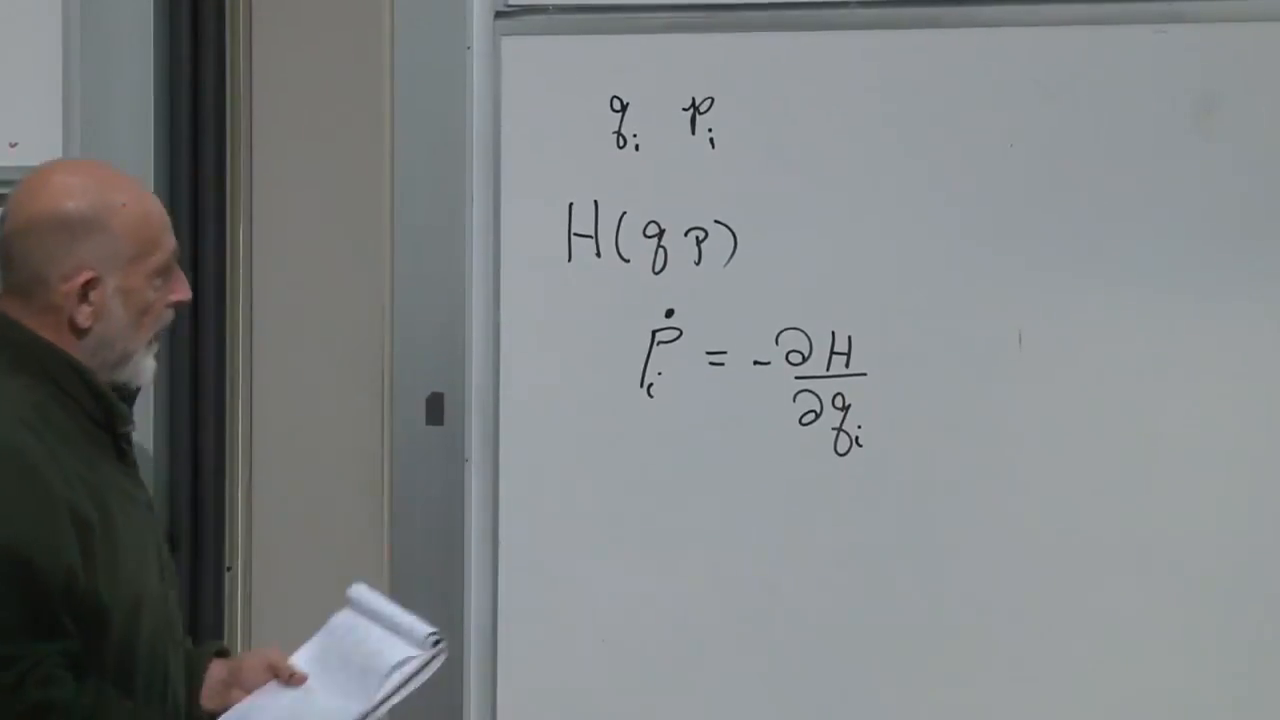
\includegraphics[width=0.82\textwidth]{lecture_07_figure_02.png}
  \caption{복습의 도입부에 제시된 정준변수와 함수 \(H(q,p)\), 그리고 운동량에 관한 해밀턴 방정식.}
  \lectureframe{00:07:29}
\end{figure}

방정식은 지표가 붙은 쌍으로 주어지지만, 운동이 쌍마다 분리될 필요는 없다. 해밀토니안은 모든 \(q_i\)와 \(p_i\)를 서로 결합할 수 있으므로, 예를 들어 \(\dot p_1\)는 계 전체의 상태에 의존할 수 있다.

\begin{classroomqa}
  \audiencequestion{이제 설명이 공리적이 되었나요? \(p\)와 \(q\) 사이의 어떤 관계를 가정했나요?
  \lecturetimestamp{00:17:08--00:18:18}}
  \lecturerresponse{\(H(q,p)\)와 정준 좌표쌍을 지정하면 해밀턴 방정식으로 형식 이론이 정의된다. 보편적으로 추가되는 가정 \(p=m\dot q\)은 없다. 이 관계는 운동에너지가 이차식인 보통의 데카르트 좌표계 입자에서는 성립하지만, 좌표나 해밀토니안이 달라지면 운동량--속도 관계도 달라진다. 그 관계는 방정식 자체에서 \(\dot q_i=\partial H/\partial p_i\)를 통해 주어진다. 제안된 해밀토니안이 자연에서 실현되는지는 별도의 물리적 문제다.}
\end{classroomqa}

이제 한 줄의 논리로 에너지 보존을 되짚어 볼 수 있다. 궤적을 따라 \(H\)의 전미분은 다음과 같다.
\begin{equation}
  \frac{dH}{dt}
  =
  \sum_i\left(
    \frac{\partial H}{\partial q_i}\dot q_i
    +\frac{\partial H}{\partial p_i}\dot p_i
  \right)
  +\frac{\partial H}{\partial t}.
  \label{eq:l7-total-h-derivative}
\end{equation}
마지막 항은 \(q\)와 \(p\)를 고정했을 때의 명시적 시간 의존성을 뜻한다. 외부에서 지정한 매개변수가 변하는 경우가 그 예다. 식~\eqref{eq:l7-hamilton-equations}을 대입하면,
\begin{align}
  \frac{dH}{dt}
  &=
  \sum_i\left[
    \frac{\partial H}{\partial q_i}
    \frac{\partial H}{\partial p_i}
    -\frac{\partial H}{\partial p_i}
    \frac{\partial H}{\partial q_i}
  \right]
  +\frac{\partial H}{\partial t}\\
  &=\frac{\partial H}{\partial t}.
  \label{eq:l7-h-energy-rate}
\end{align}
합의 각 항은 짝이 되는 항과 상쇄된다. 따라서
\begin{equation}
  \frac{\partial H}{\partial t}=0
  \quad\Longrightarrow\quad
  \frac{dH}{dt}=0.
  \label{eq:l7-energy-conservation}
\end{equation}
시간 병진 대칭성을 갖는 닫힌계에서는 해밀토니안이 보존되며, 이것이 에너지다.

\begin{classroomqa}
  \audiencequestion{해밀토니안이 시간에 명시적으로 의존하면 무엇이 달라지나요? \lecturetimestamp{00:10:32--00:12:33}}
  \lecturerresponse{그러면 식~\eqref{eq:l7-h-energy-rate}은 여전히 성립하지만, 부분계의 에너지는 일정하지 않을 수 있다. 명시적 시간 의존성은 대개 계와 에너지를 주고받는 외부 구동원이 생략되어 있음을 나타낸다. 그 구동원을 더 큰 닫힌계의 동역학적 일부로 포함하면, 더 큰 계의 해밀토니안은 다시 시간에 무관해질 수 있고 전체 에너지도 보존된다.}
\end{classroomqa}

\section{위상 공간의 기하로 보는 에너지}

이제 \(H\)가 시간에 명시적으로 의존하지 않는다고 하자. 초기 조건에 따라 값 \(E\)가 정해지고, 위상점은 \begin{equation}
  H(q,p)=E.
  \label{eq:l7-energy-surface}
\end{equation} 위에 머문다.
위상 공간의 차원은 \(2n\)이다. 정칙점에서는 좌표들 사이의 방정식 하나가 \((2n-1)\)차원 초곡면을 정의한다. \(E\)의 값이 다르면 서로 다른 초곡면이 주어진다. 이 초곡면이 닫혀 있거나 유계일 필요는 없다. 에너지 보존이 말해 주는 것은 그중 하나에서 시작한 궤적이 그 초곡면을 벗어나지 않는다는 것뿐이다.

앞 강의에서 다룬 조화진동자의 정준화된 형식에서는,
\begin{equation}
  H=\frac{\omega}{2}(p^2+q^2).
  \label{eq:l7-oscillator-hamiltonian}
\end{equation}
따라서 각 일정 에너지 집합은 원이다.
\begin{equation}
  p^2+q^2=\frac{2E}{\omega}.
  \label{eq:l7-oscillator-circle}
\end{equation}

\begin{figure}[htbp]
  \centering
  \includegraphics[width=0.84\textwidth]{lecture_07_figure_04.png}
  \caption{\(2n\)차원 위상공간 도식과 일정 에너지 곡면을 도입할 때 사용한 조화진동자의 해밀토니안.}
  \lectureframe{00:15:20}
\end{figure}

운동 방정식은
\begin{equation}
  \dot q=\omega p,\qquad \dot p=-\omega q,
  \label{eq:l7-oscillator-flow}
\end{equation}
위상점을 해당 원을 따라 시계 방향으로 움직인다. 에너지 방정식은 운동이 놓이는 곡선을 알려 주고, 해밀턴 방정식은 그 곡선을 따라가는 방향과 속력을 알려 준다.

\begin{figure}[htbp]
  \centering
  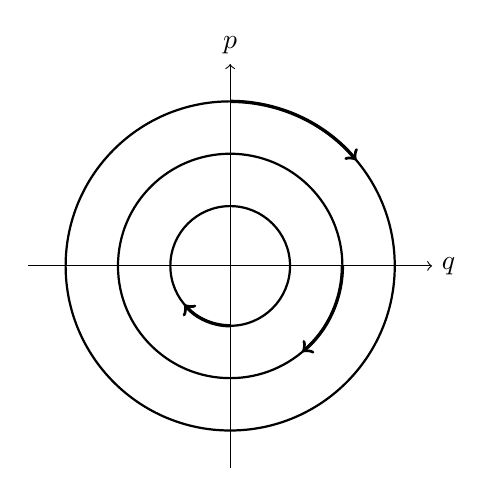
\begin{tikzpicture}[scale=0.95]
    \draw[->] (-2.7,0) -- (2.7,0) node[right] {\(q\)};
    \draw[->] (0,-2.7) -- (0,2.7) node[above] {\(p\)};
    \draw[thick] (0,0) circle (0.8);
    \draw[thick] (0,0) circle (1.5);
    \draw[thick] (0,0) circle (2.2);
    \draw[->,very thick] (0,2.2) arc[start angle=90,end angle=40,radius=2.2];
    \draw[->,very thick] (1.5,0) arc[start angle=0,end angle=-50,radius=1.5];
    \draw[->,very thick] (0,-0.8) arc[start angle=-90,end angle=-140,radius=0.8];
  \end{tikzpicture}
  \caption{일정한 에너지가 원들을 정하고, 진동자 방정식이 시계 방향 접선 흐름을 정한다.}
\end{figure}

\begin{classroomqa}
  \audiencequestion{해밀턴 방정식 두 개와 \(H=E\)는 같은 방정식을 달리 쓴 것인가요?
  \lecturetimestamp{00:15:53--00:17:06}}
  \lecturerresponse{아니다. 해밀턴 방정식은 정준 좌표쌍 하나에 대한 1계 운동 법칙 두 개다. 이 방정식들로부터 \(dH/dt=0\)가 나오고, 여기서 \(H=E\)가 따른다. \(E\)의 값은 초기 조건으로 정해진다. 방정식 \(H=E\)은 곡면을 지정할 뿐, 그 곡면을 따라가는 속도를 그 자체로 정하지는 않는다.}
\end{classroomqa}

\section{한 상태에서 상태들의 흐름으로}

초기 조건 하나를 따라가는 대신, 가능한 모든 초기 조건을 위상 공간에 뿌려 놓고 시간을 흘려 보자. 각 점은 완전한 가능한 상태 하나이며, 각 상태는 해밀턴 방정식에 따라 움직인다. 이 점들의 분포는 먼지나 가상의 유체로 상상할 수 있다. 실제 물질을 위상 공간에 쏟아붓는 것은 아니다. 이 유체는 모든 궤적을 한꺼번에 살펴보기 위한 표현이다.

위상 공간의 속도장은
\begin{equation}
  \mathbf V(q,p,t)
  =
  (\dot q_1,\ldots,\dot q_n,\dot p_1,\ldots,\dot p_n).
  \label{eq:l7-phase-velocity}
\end{equation}
정준 좌표쌍 하나에 대해서는 다음과 같이 쓴다.
\begin{equation}
  V_q=\dot q=\frac{\partial H}{\partial p},
  \qquad
  V_p=\dot p=-\frac{\partial H}{\partial q}.
  \label{eq:l7-phase-components}
\end{equation}
해밀토니안은 각 점에서 위상점을 다음에 어디로 보낼지 나타내는 벡터를 정한다. \(H\)가 시간에 무관하면 벡터장은 정상 상태다. 같은 위상점으로 돌아오면 같은 속도를 얻는다. \(H\)가 시간에 의존하면 벡터장 자체가 시간에 따라 변하지만, 그래도 매 순간 정의된다.

\begin{figure}[htbp]
  \centering
  \includegraphics[width=0.84\textwidth]{lecture_07_figure_05.png}
  \caption{조화진동자의 속도장. 벡터는 원에 접하며 원점에 가까울수록 짧아진다.}
  \lectureframe{00:24:50}
\end{figure}

조화진동자에서는 모든 반지름이 각속력 \(\omega\)로 회전한다. 원점에 가까운 점은 같은 주기 동안 더 짧은 원을 따라가므로 선속력이 더 작다. 따라서 먼지 전체는 강체 회전목마처럼 회전한다.

\begin{classroomqa}
  \audiencequestion{강체 회전이라면 모든 조화진동자 궤도의 주기가 같은가요? \lecturetimestamp{00:21:10--00:21:42}}
  \lecturerresponse{그렇다. 진폭과 무관하다는 점이 조화진동자를 특징짓는 특별한 성질이다. 위상 공간 속도 벡터의 크기는 작은 원일수록 작지만, 모든 원을 같은 각진동수 \(\omega\)로 돈다.}
\end{classroomqa}

\begin{classroomqa}
  \audiencequestion{위상 공간의 속도는 모든 점에서 같은가요?
  \lecturetimestamp{00:24:29--00:25:37}}
  \lecturerresponse{아니다. 방향과 크기는 일반적으로 위치에 따라 달라진다. 조화진동자에서 벡터는 그 점의 원에 접하며 크기는 \(\omega\sqrt{p^2+q^2}\)이다. 벡터장이란 모든 점에 각각 하나씩 벡터를 지정한 것이지, 똑같은 벡터 하나를 모든 곳에 복사한 것이 아니다.}
\end{classroomqa}

\begin{classroomqa}
  \audiencequestion{이 가상 유체의 입자와 밀도는 정확히 무엇을 뜻하나요? \lecturetimestamp{00:56:03--00:58:40}}
  \lecturerresponse{각 점은 역학계 전체의 완전한 상태 하나를 나타낸다. 물리적 입자 하나를 뜻하는 것이 아니다. 공간 차원이 1인 곳에서 입자 5개의 상태를 나타내려면 위치 5개와 운동량 5개가 필요하므로 위상 공간은 10차원이다. 3차원 공간에서는 30차원이 필요하다. 먼지는 서로 다른 대안적 상태들의 앙상블이다. 유체 그림이 오히려 혼란스럽다면 초기 조건 영역 하나를 잡아 그 안의 모든 점을 시간에 따라 진화시키고, 전후의 위상 공간 부피를 비교하면 된다.}
\end{classroomqa}

\section{압축과 발산}

이 가상 유체의 부피가 줄어드는지 알아보려면 1차원에서 시작하자. 직선 위의 점들이 속도 \(v(x)\)로 움직인다고 하자. \(\delta x\)만큼 떨어진 두 점 사이의 속도 차는
\begin{equation}
  \delta v \simeq \frac{dv}{dx}\,\delta x.
  \label{eq:l7-one-dimensional-strain}
\end{equation}
\(dv/dx>0\)이면 앞쪽 점이 더 빠르게 움직여 구간이 늘어난다. \(dv/dx<0\)이면 구간은 압축된다. 따라서 정상 1차원 비압축성 흐름은
\begin{equation}
  \frac{dv}{dx}=0.
  \label{eq:l7-one-dimensional-incompressible}
\end{equation}

\begin{figure}[htbp]
  \centering
  \includegraphics[width=0.84\textwidth]{lecture_07_figure_06.png}
  \caption{\(dv/dx\)를 국소적인 늘어남 또는 압축률로 도입하는 1차원 구성.}
  \lectureframe{00:30:20}
\end{figure}

서로 동등한 관점이 두 가지 있다. 물질 구간을 따라가며 길이가 변하는지 살펴볼 수 있다. 또는 작은 구간을 고정해 놓고 단위 시간당 들어오는 양과 나가는 양이 같은지 물을 수 있다. 첫 번째는 유체를 따라가고, 두 번째는 유체가 지나가는 모습을 관찰한다.

여러 차원에서는 전체 부피가 변하지 않으면서 한 축을 따라 영역이 늘어나고 다른 축을 따라 압축될 수 있다. 속도장 \(\mathbf V=(V_x,V_y,V_z)\)에 대해 관련된 국소 변화율은 발산이다.
\begin{equation}
  \nabla\cdot\mathbf V
  =
  \frac{\partial V_x}{\partial x}
  +\frac{\partial V_y}{\partial y}
  +\frac{\partial V_z}{\partial z}.
  \label{eq:l7-spatial-divergence}
\end{equation}
발산이 양수이면 국소적으로 팽창하고, 음수이면 국소적으로 수축하며, 비압축성 조건은
\begin{equation}
  \nabla\cdot\mathbf V=0.
  \label{eq:l7-zero-divergence}
\end{equation}
고정된 작은 상자를 드나드는 유량이 같은 것은 움직이는 작은 상자의 부피가 보존된다는 것과 동일한 국소적 진술이다.

\begin{figure}[htbp]
  \centering
  \includegraphics[width=0.86\textwidth]{lecture_07_figure_07.png}
  \caption{2차원 상자와 그 흐름 성분, 그리고 발산을 정의하는 동일 좌표에 대한 미분들의 합.}
  \lectureframe{00:35:30}
\end{figure}

\begin{classroomqa}
  \audiencequestion{보통 공간의 유체를 다루는 건가요, 위상 공간의 흐름을 다루는 건가요? \lecturetimestamp{00:34:27--00:34:40}}
  \lecturerresponse{발산 논증은 우선 일반적인 유체 논증이다. 이제 이를 차원이 짝수인 위상 공간에 적용할 것이다. 이 공간에서 좌표 방향은 \(q_i\)와 \(p_i\)이고 속도 성분은 \(\dot q_i\)와 \(\dot p_i\)이다.}
\end{classroomqa}

이제 이산 상태 사상으로 돌아가자. 가역 순환에서는 각 노드에 들어오는 화살표와 나가는 화살표가 하나씩 있으며, 선택한 상태들의 집합은 진화해도 원소 수를 그대로 유지한다. 흡인점에서는 들어오는 화살표가 많고 나가는 화살표는 너무 적다. 여러 대안이 서로 구분되지 않게 된다.

\begin{figure}[htbp]
  \centering
  \includegraphics[width=0.80\textwidth]{lecture_07_figure_08.png}
  \caption{발산 개념을 첫 강의의 가역 법칙 판별 기준과 다시 연결하는 이산 흡인점.}
  \lectureframe{00:40:15}
\end{figure}

이제 연속적인 경우의 질문을 정확히 할 수 있다. 해밀턴 흐름의 발산이 0이어서, 구분 가능한 상태들의 작은 영역이 더 작은 위상 공간 부피로 뭉개지지 않는가?

\section{리우빌 정리}

\begin{theorem}[Liouville's theorem]매끄러운 해밀턴 계에서 정준 위상 공간 속도장의 발산은 0이다.
\begin{equation}
  \sum_i\left(
    \frac{\partial\dot q_i}{\partial q_i}
    +\frac{\partial\dot p_i}{\partial p_i}
  \right)=0.
  \label{eq:l7-liouville-divergence}
\end{equation}
따라서 해밀턴 시간발전은 정준 위상 공간 부피 \(dq_1\cdots dq_n\,dp_1\cdots dp_n\)를 보존한다.
\end{theorem}

\begin{classroomqa}
  \audiencequestion{성분 \(V\)은 단순히 \(p\)의 시간미분과 \(q\)의 시간미분인가요? \lecturetimestamp{00:42:20--00:43:22}}
  \lecturerresponse{그렇다. 정준 좌표쌍 하나에 대해서는 \(V_q=\dot q\)이고 \(V_p=\dot p\)이다. 이 미분들을 모두 배열하면 전체 위상 공간에서 흐름의 속도 벡터가 된다.}
\end{classroomqa}

정준 좌표쌍 하나에 대해 해밀턴 방정식은
\begin{equation}
  V_p=-\frac{\partial H}{\partial q},
  \qquad
  V_q=\frac{\partial H}{\partial p}.
  \label{eq:l7-liouville-components}
\end{equation}
따라서 발산은
\begin{align}
  \frac{\partial V_p}{\partial p}
  +\frac{\partial V_q}{\partial q}
  &=
  -\frac{\partial}{\partial p}
    \left(\frac{\partial H}{\partial q}\right)
  +\frac{\partial}{\partial q}
    \left(\frac{\partial H}{\partial p}\right)\\
  &=
  -\frac{\partial^2H}{\partial p\,\partial q}
  +\frac{\partial^2H}{\partial q\,\partial p}
  =0.
  \label{eq:l7-liouville-proof}
\end{align}

\begin{figure}[htbp]
  \centering
  \includegraphics[width=0.86\textwidth]{lecture_07_figure_09.png}
  \caption{매끄러운 혼합 편미분이 교환됨을 설명하는 유한 차분 사각형.}
  \lectureframe{00:47:30}
\end{figure}

혼합 편미분의 등식은 \(A,B,C,D\)가 \(q\)-\(p\) 평면의 작은 사각형 꼭짓점에 놓인 경우를 통해 볼 수 있다. \(q\)에 대해 유한 차분을 취한 다음 \(p\)에 대해 유한 차분을 취하면, 두 변의 작은 길이를 곱한 인자를 제외하고
\begin{equation}
  F(B)+F(D)-F(A)-F(C).
  \label{eq:l7-finite-difference-combination}
\end{equation}
차분의 순서를 반대로 해도 같은 조합이 나온다. 작은 사각형 극한에서는 필요한 미분들이 연속인 경우
\(\partial_p\partial_qF=\partial_q\partial_pF\)이다.

\begin{figure}[htbp]
  \centering
  \includegraphics[width=0.88\textwidth]{lecture_07_figure_10.png}
  \caption{해밀턴 방정식으로부터 부호가 반대인 두 혼합 미분으로 정리된 정준 발산.}
  \lectureframe{00:50:20}
\end{figure}

자유도가 많아도 모든 정준 좌표쌍에서 같은 상쇄가 일어난다.
\begin{align}
  \sum_i\left(
    \frac{\partial\dot p_i}{\partial p_i}
    +\frac{\partial\dot q_i}{\partial q_i}
  \right)
  &=
  \sum_i\left(
    -\frac{\partial^2H}{\partial p_i\,\partial q_i}
    +\frac{\partial^2H}{\partial q_i\,\partial p_i}
  \right)\\
  &=0.
  \label{eq:l7-many-pair-proof}
\end{align}
한 정준 방향의 신장은 그 켤레 방향의 압축으로 상쇄된다. 이렇게 좌표쌍마다 일어나는 상쇄는 서로 관련 없는 축들 사이의 우연한 상쇄보다 더 강한 구조를 보여 준다.

\begin{classroomqa}
  \audiencequestion{모든 정준 좌표쌍에 대해 합을 취한다고 이해하면 되나요?
  \lecturetimestamp{00:52:00--00:52:36}}
  \lecturerresponse{그렇다. 식~\eqref{eq:l7-many-pair-proof}은 \(i\)에 대해 합을 취하며, 각 \(q_i,p_i\) 쌍 안에서 두 혼합 미분이 따로 상쇄된다.}
\end{classroomqa}

\begin{classroomqa}
  \audiencequestion{표시된 발산은 데카르트 좌표계의 형태로 보입니다. 좌표를 바꾸어도 정리는 성립하나요?
  \lecturetimestamp{00:52:50--00:53:22,\allowbreak\ 00:58:18--00:58:40}}
  \lecturerresponse{자연스러운 진술은 정준 좌표와 정준 부피 요소 \(dq_1\cdots dq_n\,dp_1\cdots dp_n\)를 사용한다. 정준 변환, 즉 심플렉틱 변환은 좌표와 운동량을 함께 바꾸며 이 부피를 보존한다. 정준이 아닌 임의의 좌표계에서는 부피 측도에 야코비 인자가 포함된다. 따라서 좌표 미소량을 단순히 곱한 값은 불변량일 필요가 없다.}
\end{classroomqa}

\begin{classroomqa}
  \audiencequestion{리우빌 정리는 시간에 무관한 해밀토니안을 필요로 하나요? \lecturetimestamp{00:53:43--00:55:51}}
  \lecturerresponse{아니다. 에너지 보존에는 \(\partial H/\partial t=0\)가 필요하지만, 발산 증명에서는 고정된 시각에 \(q_i\)와 \(p_i\)에 대해서만 미분한다. \(H(q,p,t)\)일 때 혼합 편미분은 여전히 상쇄된다. 따라서 시간에 의존하는 해밀토니안도 시간에 따라 변하지만 매 순간 부피를 보존하는 정준 흐름을 만든다.}
\end{classroomqa}

\section{부피 보존이 뜻하는 것과 뜻하지 않는 것}

초기 조건의 작은 영역 \(R_0\)을 잡고 그 안의 모든 점을 시간 \(t\) 동안 진화시키자. 리우빌 정리에 따르면
\begin{equation}
  \operatorname{Vol}(R_t)=\operatorname{Vol}(R_0).
  \label{eq:l7-volume-preservation}
\end{equation}
영역은 이동하고, 회전하고, 전단되어 긴 실 모양으로 늘어날 수 있다. 보존되는 것은 모양이 아니라 부피다. 매끄러운 해밀턴 시간발전이 유한한 시간 동안 서로 다른 위상점들을 하나로 합치지는 않는다.

유한한 시간 동안 매끄러운 해밀턴 흐름은 가역 사상이며, 역방향으로 시간발전시켜 매끄러운 역함수를 얻을 수 있다. 이 점은 연결된 덩어리가 두 개의 서로 떨어진 조각으로 잘려 나갈 수 없다는 강의의 설명도 뒷받침한다. 흐름은 영역을 연속적으로 변형하며 위상을 보존한다. 다만 목 부분이 극도로 가늘어지면 유한한 해상도에서는 두 엽이 분리된 것처럼 보일 수 있다.

\begin{figure}[htbp]
  \centering
  \includegraphics[width=0.86\textwidth]{lecture_07_figure_12.png}
  \caption{위상 공간 영역의 가능한 변형. 매끄러운 해밀턴 흐름은 가느다란 목을 만들 수 있지만, 유한한 시간 안에 영역이 실제로 끊어져 서로 독립적으로 진화하는 조각들로 나뉘게 할 수는 없다.}
  \lectureframe{01:04:55}
\end{figure}

\begin{classroomqa}
  \audiencequestion{위상 공간의 영역이 끊어져 두 조각으로 나뉠 수 있나요? \lecturetimestamp{01:04:10--01:05:49}}
  \lecturerresponse{매끄러운 결정론적 해밀턴 흐름에서는 유한한 시간 동안 그렇게 되지 않는다. 가상의 끊김 점에도 위상점 하나와 그 점에 지정된 속도 하나가 있다. 서로 양립하지 않는 두 방향이 있는 것이 아니다. 영역은 아주 길고 가느다란 연결 실 모양으로 변할 수 있지만, 시간발전은 일대일 대응을 유지하며 그 영역을 찢지 않는다.}
\end{classroomqa}

\begin{classroomqa}
  \audiencequestion{늘어난 덩어리의 서로 멀리 떨어진 두 엽은 물리적으로 연결되어 있거나 양자 얽혀 있나요?
  \lecturetimestamp{01:08:01--01:09:16}}
  \lecturerresponse{그런 물리적 연결을 뜻하지 않는다. 덩어리는 하나의 물질적 대상이 아니라 대안적인 초기 조건들의 집합이다. 이를 하나의 영역이라고 부르는 것은 그 상태들이 공통된 집합에서 진화했음을 나타낼 뿐, 그들 사이에 힘이나 양자 얽힘이 있음을 뜻하지 않는다.}
\end{classroomqa}

\begin{classroomqa}
  \audiencequestion{강체 진자의 불안정한 수직 평형점 근처에서는 어떤 일이 일어나나요? 시계 방향 궤도와 반시계 방향 궤도가 겹치나요?
  \lecturetimestamp{01:07:07--01:07:47}}
  \lecturerresponse{가까운 초기 조건들이 서로 크게 다른 궤도로 갈라지며, 앞서 설명한 가느다란 실 모양을 만들 수 있다. 하지만 같은 위상점이 되지는 않는다. 무한소 변위나 운동량의 부호가 양쪽을 구분한다. 정확히 균형 잡힌 상태에는 고유하게 정해지는 운동이 따르는데, 이상적인 모형에서는 평형 상태에 계속 머무는 것이다.}
\end{classroomqa}

\subsection{위치 공간의 팽창과 운동량 공간의 수축}

정준 변환이 위치 범위를 \(a\)배 늘리면 켤레 운동량의 척도는 그 역수만큼 줄어든다.
\begin{equation}
  q\longrightarrow aq,
  \qquad
  p\longrightarrow \frac{p}{a},
  \qquad
  dq\,dp\longrightarrow dq\,dp.
  \label{eq:l7-canonical-scaling}
\end{equation}
이것이 기체 팽창 사례의 위상 공간에서의 명확한 의미다. 단열 팽창에서는 접근 가능한 보통 공간의 영역이 커지는 한편, 전형적인 운동량은 작아지고 기체는 냉각된다. 구체적인 열역학 관계는 차원, 팽창 방식, 상호작용에 따라 달라진다. 리우빌 정리는 부피 제약을 제공할 뿐, 모든 열역학 계수를 정해 주지는 않는다.

\begin{classroomqa}
  \audiencequestion{급격한 팽창의 경우에도 같은 논리가 적용되나요? 팽창하는 우주에도 해당하나요? \lecturetimestamp{00:53:23--00:56:00}}
  \lecturerresponse{완전한 동역학이 해밀턴 형식이면 명시적으로 시간에 의존하는 정준 변수의 경우를 포함해 리우빌 정리가 적용된다. 위치 방향의 팽창에는 그에 대응하는 정준 운동량 방향의 수축이 따라야 한다. 그러나 우주론적 척도인자, 제어된 기체 팽창, 자유롭게 폭발하는 구름은 같은 물리 과정이 아니다. 거리와 후퇴 속도 사이의 허블형 상관은 더 빠른 물체가 더 멀리 이동해서 생길 수 있다. 반면 단열 냉각은 국소 운동량 분포의 수축과 관련된다. 어느 경우든 정리는 전체 위상 공간 사상을 제약한다.}
\end{classroomqa}

\begin{classroomqa}
  \audiencequestion{리우빌 정리는 실제로 어떻게 쓰이나요?
  \lecturetimestamp{01:06:16--01:07:04}}
  \lecturerresponse{통계역학의 핵심 정리다. 미시 상태들의 앙상블이 어떻게 진화하는지를 제약하고, 위상 공간 부피와 엔트로피의 관계를 뒷받침한다. 기체의 팽창과 냉각이 바로 떠올릴 수 있는 예이며, 뒤에서는 평형 및 비평형 현상을 추론하는 기본 도구가 된다.}
\end{classroomqa}

\section{격렬하게 모양을 바꾸는 흐름}

조화진동자의 흐름은 강체 회전이므로 넓이와 모양을 모두 보존한다. 이는 특별한 경우다. 부피 보존과 강체성을 구별하기 위해 다음을 생각하자.
\begin{equation}
  H=\lambda pq,
  \label{eq:l7-pq-hamiltonian}
\end{equation}
여기서 \(\lambda\)는 시간의 역수 단위를 갖는다. 강의에서는 \(\lambda=1\)로 둔다. 이 인자를 남겨 두면 차원이 명확해진다.

\begin{figure}[htbp]
  \centering
  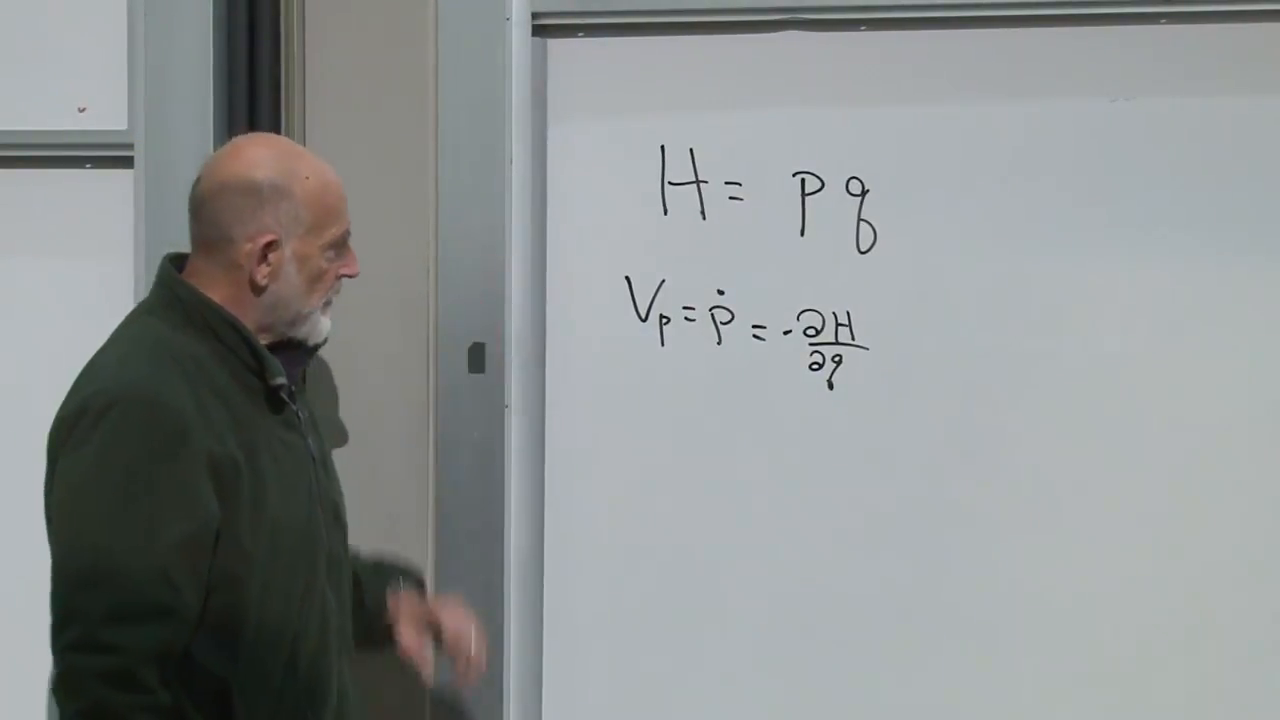
\includegraphics[width=0.82\textwidth]{lecture_07_figure_03.png}
  \caption{예제 \(H=pq\)의 시작 부분과 첫 번째 위상 공간 속도 성분.}
  \lectureframe{01:00:11}
\end{figure}

해밀턴 방정식은
\begin{equation}
  \dot p=-\lambda p,
  \qquad
  \dot q=\lambda q,
  \label{eq:l7-pq-flow}
\end{equation}
이며, 해는
\begin{equation}
  p(t)=p_0e^{-\lambda t},
  \qquad
  q(t)=q_0e^{\lambda t}.
  \label{eq:l7-pq-solutions}
\end{equation}
이다. 정사각형 패치는 \(p\) 방향으로 지수적으로 압축되고, 같은 인자만큼 \(q\) 방향으로 늘어난다.
\begin{equation}
  \Delta p(t)\Delta q(t)
  =
  \Delta p(0)\Delta q(0).
  \label{eq:l7-pq-area}
\end{equation}
발산을 계산해도 국소적으로 같은 결과를 확인할 수 있다.
\begin{equation}
  \frac{\partial\dot p}{\partial p}
  +\frac{\partial\dot q}{\partial q}
  =-\lambda+\lambda=0.
  \label{eq:l7-pq-divergence}
\end{equation}

\begin{figure}[htbp]
  \centering
  \includegraphics[width=0.86\textwidth]{lecture_07_figure_11.png}
  \caption{\(H=pq\) 흐름 아래에서 넓이를 보존하면서 길고 가느다란 띠로 늘어난 작은 패치.}
  \lectureframe{01:02:10}
\end{figure}

\begin{classroomqa}
  \audiencequestion{\(pq\)는 작용의 차원을 가지는데, 리우빌 정리는 작용 보존을 뜻하나요?\lecturetimestamp{01:03:00--01:04:09}}
  \lecturerresponse{아니다. 정리가 보존하는 것은 위상 공간 부피다. 정준 좌표쌍 하나에서 \(dq\,dp\)는 작용의 차원을 가지며, 이 차원적 사실은 위상 공간 셀의 크기를 \(\hbar\)가 정하는 양자역학을 예고한다. 그러나 곱 \(pq\) 자체는 해밀턴의 작용 범함수가 아니며, 차원이 같다는 이유만으로 각운동량이 되는 것도 아니다.}
\end{classroomqa}

이 예는 각도도 보존되지 않을 수 있음을 보여 준다. 식~\eqref{eq:l7-pq-solutions}의 스케일링 아래 성분들이 서로 다르게 변하는 직각 십자 모양은 계량상 전단되지만, 넓이는 그대로 유지된다. 리우빌 정리는 넓이 또는 부피에 관한 정리이지, 보통의 유클리드 강체성에 관한 정리가 아니다.

\section{감쇠는 흡인점을 만든다}

정리가 배제하는 것을 보려면 감쇠 진동자의 축약된 방정식을 살펴보자.
\begin{equation}
  m\ddot x=-kx-c\dot x,
  \qquad c>0.
  \label{eq:l7-damped-newton}
\end{equation}
\(p=m\dot x\)라 두면,
\begin{equation}
  \dot x=\frac{p}{m},
  \qquad
  \dot p=-kx-\frac{c}{m}p.
  \label{eq:l7-damped-first-order}
\end{equation}
감쇠가 없으면 위상점은 원점을 중심으로 돈다. 감쇠가 있으면 에너지가 주위 매질의 미시적 자유도로 전달되고 궤도는 안쪽으로 감긴다.

\begin{figure}[htbp]
  \centering
  \includegraphics[width=0.84\textwidth]{lecture_07_figure_13.png}
  \caption{감쇠 진동자의 방정식과 \(x\)-\(p\) 평면에서 안쪽으로 감기는 나선 궤도.}
  \lectureframe{01:13:30}
\end{figure}

이 2차원 축약 흐름의 발산은
\begin{equation}
  \frac{\partial\dot x}{\partial x}
  +\frac{\partial\dot p}{\partial p}
  =
  0-\frac{c}{m}<0.
  \label{eq:l7-damped-divergence}
\end{equation}
이다. 모든 유한한 패치는 수축한다. 원점은 흡인점이며, 연속적인 경우에 여러 화살표가 들어오는 상태에 해당한다.

\begin{figure}[htbp]
  \centering
  \includegraphics[width=0.88\textwidth]{lecture_07_figure_14.png}
  \caption{음의 발산 \(-c/m\)을 얻는 데 사용한 감쇠 위상 공간의 속도 성분.}
  \lectureframe{01:16:05}
\end{figure}

이는 미시적 역학이 리우빌 정리를 위반한다는 뜻이 아니다. 두 변수 \(x,p\)는 진동자의 에너지를 받아들이는 환경의 엄청난 수의 자유도를 생략한다. 진동자와 환경을 합친 확장 계는 해밀턴 계로서 부피를 보존할 수 있지만, 그 축약된 \(x,p\) 기술에서는 부피가 수축한다.

\begin{classroomqa}
  \audiencequestion{감쇠 진동자는 축약된 위상 공간에서 해밀턴 계가 아닌데도 여전히 뉴턴 방정식으로 기술되는가?
  \lecturetimestamp{01:20:09--01:21:12}}
  \lecturerresponse{그렇다. 뉴턴의 \(F=ma\)에는 경험적으로 주어지는 항력도 포함될 수 있다. 기본적인 \(L=T-V\) 및 해밀턴 기술은 보존력에 직접 적용되며, 더 일반적인 라그랑지안은 속도에 의존하는 힘의 일부도 다룬다. 그러나 고립된 한 쌍 \(x,p\)에 대한 마르코프 마찰항은 축약된 소산 동역학이지, 닫힌 정준 해밀턴 계가 아니다.}
\end{classroomqa}

\begin{classroomqa}
  \audiencequestion{감쇠 방정식을 무한한 정밀도로 역방향 적분할 수 있다면, 정보는 정말로 사라지는가?
  \lecturetimestamp{01:25:16--01:27:17}}
  \lecturerresponse{유한한 시간 동안에는 이상적인 미분 방정식에 여전히 역변환이 있으므로 정확한 자료를 역방향으로 계산할 수 있다. 정확한 진술은 유한한 위상 공간 셀의 부피가 지수적으로 수축한다는 것이다. 따라서 과거 상태를 복원하려면 정밀도를 지수적으로 높여야 하며, 무한한 시간이 지나면 모든 궤적은 흡인점에 접근한다. 이는 이산적인 대안 소실 그림에 가장 가까운 연속 고전적 유비이지, 유한한 시간 안에 두 정확한 해가 문자 그대로 하나가 된다는 주장은 아니다.}
\end{classroomqa}

\begin{classroomqa}
  \audiencequestion{발산이 0인 벡터장이 해밀턴 형식에서 나오지 않을 수도 있는가? \lecturetimestamp{01:18:21--01:22:34}}
  \lecturerresponse{물론이다. 해밀턴 형식은 발산이 0이 되기에 충분하지만 필수 조건은 아니다. 임의의 비압축성 속도장은 같은 공간에서 정준 해밀턴 벡터장이 아니더라도 발산이 0일 수 있다. 3차원 비압축성 유체의 속도장이 교과서적인 예다. 세 좌표만으로는 정준 쌍을 이룰 수 없다. 유체 역학 전체에는 더 정교한 무한 차원 해밀턴 형식이 존재할 수 있지만, 그렇다고 여기서 말한 한 방향의 함의가 뒤집히는 것은 아니다.}
\end{classroomqa}

\section{질문을 통해 드러나는 추가적인 구분}

\begin{classroomqa}
  \audiencequestion{일정한 에너지 곡면 위의 운동은 위상 공간 전체 부피의 보존과 어떤 관계가 있는가?
  \lecturetimestamp{01:28:47--01:30:41}}
  \lecturerresponse{두 현상은 해밀턴 구조에서 독립적으로 따르는 결과다. \(H\)가 시간에 명시적으로 의존하지 않으면, 각 궤적은 자기 에너지 곡면 위에 머문다. 유한한 영역은 여러 에너지 곡면을 가로지를 수 있지만, 리우빌 정리는 그 영역 전체의 부피가 보존된다고 말한다. 조화 진동자의 경우에는 흐름이 강체 회전이므로 영역의 모양도 유지된다. \(H=pq\) 영역은 넓이만 유지하고 모양은 유지하지 않는다.}
\end{classroomqa}

\begin{classroomqa}
  \audiencequestion{해밀턴 기술에서 역학적 일은 어떻게 다루는가? \lecturetimestamp{01:30:44--01:32:57}}
  \lecturerresponse{일은 선택한 계의 경계를 넘어 전달되는 에너지를 기술한다. 외부 작용자가 추를 들어 올리거나 매개변수를 바꾸어 부분계의 에너지를 변화시킬 수 있으며, 이때 공급한 에너지만큼 작용자의 에너지는 감소한다. 양쪽을 하나의 닫힌 모형에 포함하면, 초점은 전체 에너지의 보존과 부분계 사이의 에너지 교환으로 돌아간다.}
\end{classroomqa}

\begin{classroomqa}
  \audiencequestion{부피 보존은 위상과 각도도 보존하는가?
  \lecturetimestamp{01:33:00--01:33:37}}
  \lecturerresponse{매끄러운 유한 시간 해밀턴 흐름은 가역적인 연속 변형이므로 위상을 보존한다. 그러나 일반적으로 유클리드 각도나 모양은 보존하지 않는다. 진동자의 강체 회전에서는 보존되지만, \(H=pq\)의 신장은 그것이 특수한 경우임을 보여 준다.}
\end{classroomqa}

\begin{classroomqa}
  \audiencequestion{르장드르 변환은 물리적 의미가 없어서 생략되었는가?
  \lecturetimestamp{01:33:43--01:34:48}}
  \lecturerresponse{아니다. 속도 기술을 운동량 기술로 바꾸고, 사상이 정칙일 때 \(H=\sum_i p_i\dot q_i-L\)를 얻는 유용한 변환이다. 형식적인 이름을 강조하지 않았을 뿐, 이 구성은 이미 여러 차례 사용되었다. 다만 현재의 정리를 위해서는 일반 이론을 자세히 다룰 필요가 없다.}
\end{classroomqa}

\section{푸아송 괄호: 다음 단계의 압축}

마지막 몇 분 동안에는 다시 역사적 주제로 돌아간다. 19세기 역학은 겉보기에 서로 다른 계를 연결하는 간결한 구조를 거듭 모색했다---역학과 기하 광학, 입자와 광선, 고전 궤적과 파동적 기술이 그 예다. 푸아송 괄호도 그러한 구조의 하나이며, 양자역학에서 특히 중요해진다.

\(F(q,p)\)를 위상 공간 위의 임의의 함수라고 하자. 좌표나 운동량, 곱 \(qp\) 또는 각운동량일 수 있다. 운동을 따라 \begin{equation}
  \frac{dF}{dt}
  =
  \sum_i\left(
    \frac{\partial F}{\partial q_i}\dot q_i
    +\frac{\partial F}{\partial p_i}\dot p_i
  \right).
  \label{eq:l7-f-time-derivative}
\end{equation}
해밀턴 방정식을 대입하면 다음을 얻는다.
\begin{equation}
  \frac{dF}{dt}
  =
  \sum_i\left(
    \frac{\partial F}{\partial q_i}
    \frac{\partial H}{\partial p_i}
    -
    \frac{\partial F}{\partial p_i}
    \frac{\partial H}{\partial q_i}
  \right).
  \label{eq:l7-f-hamiltonian-derivative}
\end{equation}

\begin{figure}[htbp]
  \centering
  \includegraphics[width=0.88\textwidth]{lecture_07_figure_15.png}
  \caption{일반적인 위상 공간 함수 \(F(q,p)\)의 시간 미분에 대한 연쇄 법칙.}\lectureframe{01:42:40}
\end{figure}

반복해서 나타나는 반대칭 조합에 이름을 붙이자. 두 함수 \(F\)와 \(G\)의 푸아송 괄호를 다음과 같이 정의한다.
\begin{equation}
  \boxed{
  \{F,G\}
  =
  \sum_i\left(
    \frac{\partial F}{\partial q_i}
    \frac{\partial G}{\partial p_i}
    -
    \frac{\partial F}{\partial p_i}
    \frac{\partial G}{\partial q_i}
  \right).}
  \label{eq:l7-poisson-bracket}
\end{equation}

\begin{figure}[htbp]
  \centering
  \includegraphics[width=0.86\textwidth]{lecture_07_figure_16.png}
  \caption{두 함수의 미분 조합을 푸아송 괄호로 정의한 식.}\lectureframe{01:44:15}
\end{figure}

식~\eqref{eq:l7-f-hamiltonian-derivative}은 다음과 같이 된다.
\begin{equation}
  \boxed{\frac{dF}{dt}=\{F,H\}.}
  \label{eq:l7-hamiltonian-poisson-evolution}
\end{equation}
\(F\)도 시간에 명시적으로 의존하면 \(\partial F/\partial t\)를 더한다. \(F=q_i\) 또는 \(F=p_i\)를 대입하면 해밀턴의 두 방정식을 얻으므로, 식~\eqref{eq:l7-hamiltonian-poisson-evolution}은 전체 동역학을 간결하게 표현한다.

표기는 언제든 인위적으로 압축할 수 있다---여러 방정식을 제곱해 더한 뒤 하나의 방정식이라고 부를 수도 있다. 그렇게 하면 구조를 드러내기보다 감추게 된다. 푸아송 괄호가 유용한 이유는 정반대다. 푸아송 괄호의 대수 구조는 시간에 따른 변화, 보존량, 대칭을 체계화한다. 다음 단계에서는 그 대수 구조를 전개한 뒤, 고전역학과 양자 이론 모두에서 중심이 될 각운동량에 적용한다.

\section{가역성의 연속적인 의미}

이제 논리의 흐름을 줄이지 않고 진술할 수 있다. 해밀턴 방정식은 해밀토니안에 명시적인 시간 의존성이 없을 때 \(H\)를 보존하므로, 개별 궤적은 일정한 에너지 초곡면 위에 머문다. 같은 방정식은 위상 공간의 모든 점에 속도 벡터를 대응시킨다. 혼합 편미분들이 쌍으로 상쇄되므로 이 속도장의 발산은 사라진다. 따라서 가능한 상태들의 전체 영역은 정준 부피를 보존한다.

이것이 들어오는 화살표 하나와 나가는 화살표 하나에 해당하는 연속적인 경우다. 모양은 바뀔 수 있고, 각도도 바뀔 수 있으며, 이웃한 궤적들이 크게 벌어질 수도 있다. 매끄럽고 닫힌 해밀턴 기술에서는 유한한 대안들의 집합을 더 작은 위상 공간 부피로 압축할 수 없다. \(H=pq\) 흐름은 신장이 허용됨을 보여 준다. 축약된 감쇠 진동자는 해밀턴 조건을 버렸을 때 나타나는 흡인점을 보여 준다. 이어 푸아송 괄호는 해밀토니안이 모든 시간 미분을 생성한다는 진술로 같은 동역학을 압축한다.
